\section{Discussion}
\label{sec:discussion}

\subsection{What is different about a millimetre technosignature search}
\label{sec:mmdifferent}

The most transferable result of this experiment is not the non-detection but
a measurement of what limits a carrier search at these wavelengths. For
classifying a crossing in the present archival data set, molecular-line
confusion and sparse repeat coverage are more immediate limitations than
thermal sensitivity. That is a statement about disposing of events and not
about depth: the power a transmitter must radiate to be found here remains a
median $\EirpNinetySysMedA$\,W per system.

\emph{Confusion, and not interference, sets the false-positive rate.}
Catalogued molecular transitions, almost all of them carbon monoxide, account
for \NAttributed{} of the \NCross{} threshold crossings, and no crossing in
this survey is attributed to interference (Appendix~\ref{app:rfi}).
\DiscFpWin{} of the \DiscFpOfFlags{} windows that reached the spatial stage
are disc or foreground carbon monoxide, all but one the resolved disc of
$\beta$~Pictoris and the exception a cloud along the sightline to
HD~48370. The remedy that works is a
velocity-space mask evaluated in each star's own rest frame, and it is not
free: it removes \MkMaskAPct{} per cent of the
Class~A union bandwidth.

\emph{Spatially extended emission is the second discriminant, and it has no
analogue at centimetre wavelengths.} A line filling the primary beam raises
the star and the control annulus together instead of cancelling, so the
spatial statistic loses power exactly where circumstellar gas is brightest.
$\beta$~Pictoris shows the benign face: the frozen pipeline recovers its
circumstellar carbon monoxide blind, in two transitions, which is the positive
control the experiment needed. HD~48370 shows the other. Its emission ---
foreground cloud, not a disc (Appendix~\ref{app:linemask}) --- lies near a
band edge, and that one window contributes
\VnEdgeDomPct{} per cent of every near-edge threshold exceedance in the
survey: pooled, the near-edge rate is $\times\VnEdgeRatio$ the interior rate;
without that window $\times\VnEdgeNoDomRatio$, and on a held-out half
$\times\VnEdgeHalfCleanRatio$ ($\pv{\VnEdgeHalfCleanP}$). What looked like a
property of band edges is one disc, so no edge correction is applied to any
limit.

\emph{The channelisation is inherited.} \NCoarse{} of the \NWindows{} windows
have channels so coarse that every drift in the grid stays inside one channel
over a whole track; they measure an amplitude but cannot distinguish a
drifting carrier from a stationary one, which is why the carrier search rests
on \NWinA{} of them. The widths on offer here run from
\SzChanFinestKHz\,kHz to \SzChanWidestMHz\,MHz, about \SzChanDexSurvey{}
orders of magnitude; set beside the \SzChanLitHz\,Hz channels of
centimetre-band carrier searches the range becomes \SzChanDexAll{} orders
(Fig.~\ref{fig:context}(b)), and nothing in the search could choose them.

\emph{Repeat epochs turn a crossing into a testable claim, and an archive
supplies them only incidentally.} Let the \emph{confirmation coverage}
$C_{\rm conf}(\nu)$ be the number of systems toward which two independent
execution blocks more than a day apart both cover the sky frequency $\nu$, so
that a carrier found once there could have been sought again. It must be
stated against frequency rather than as a fraction of the sample, because
repeat visits re-tune and a second epoch is of no use at a frequency it does
not cover. Its support is \CvConfGHzDay\,GHz of union bandwidth,
\CvConfPctDay{} per cent of the \CvUnionA\,GHz searched, falling to
\CvConfGHzYr\,GHz beyond a year, and at its best near \CvConfNuMaxDay\,GHz it
reaches \CvConfNMaxDay{} systems (Fig.~\ref{fig:confcov}). The searched extent
is about twice the extent over which a persistent carrier could have been
confirmed, and for close to half the sample the archive constrains an
intermittent emitter hardly at all, whatever its power.

\begin{figure}
\centering
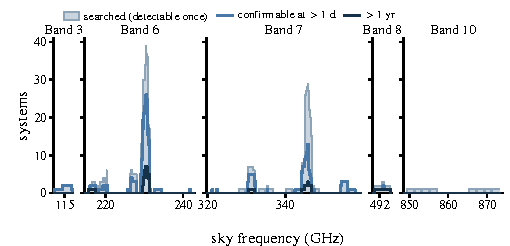
\includegraphics[width=\columnwidth]{figures/confcoverage.pdf}
\caption{What could be searched against what could be confirmed. For the
Class~A experiment, against sky frequency: the number of systems toward which
a carrier could have been detected once (grey), the number for which a second
independent execution block more than a day later also covers that frequency
(blue), and the same beyond a year (dark). One panel per populated ALMA band,
widths in proportion to the frequency each contributes, as in
Fig.~\ref{fig:covmap}.}
\label{fig:confcov}
\end{figure}

\subsection{The search space this archive opens}
\label{sec:newspace}

The carrier search is \NWinA{} fine-channel windows toward \NSysClassA{}
stellar systems, \CvUnionA\,GHz of union bandwidth; the \NWinB{}
coarse-channel windows are a supplementary spectral-excess experiment. Earlier searches above about 30\,GHz reached nearby stars at one
frequency only, and the one earlier millimetre search of comparable bandwidth
worked in Band~3 toward far more distant stars (\S\ref{sec:background}); Band~3 is searched here, in
\NWinBandThree{} windows down to \SurvFreqLo\,GHz including
$\beta$~Pictoris' CO $J=1\!-\!0$ control. Of the
\SttHayLoMHz\,MHz--\SttHayHiGHz\,GHz haystack axis of \citet{Wright2018} this
experiment covers \SttHayGHz\,GHz, only \SttHayFineGHz\,GHz of it carrier
search because the Class~A union begins at \SurvFreqLoA\,GHz; the rest lies
above that axis.

Union bandwidth overstates what that buys: different frequencies were searched
toward different numbers of stars and to very different
limits. Figure~\ref{fig:covmap} gives instead the number of independent systems
that would have yielded a recovery at ninety per cent completeness, against sky
frequency and transmitter power. At an
EIRP of $\CovEirpRefTex$\,W the covered frequency falls to
\CovUnionAtRef\,GHz, \CovFracAtRef{} per cent of the union, reaching
\CovNSysAtRef{} systems and \CovNMaxAtRef{} at the best-covered frequency near
\CovNuMaxAtRef\,GHz; with no limit on power that frequency reaches
\CovNMaxFull{} of the \NSysClassA{} systems, and half the sample only above
$\CovEirpHalf$\,W.

\begin{figure}
\centering
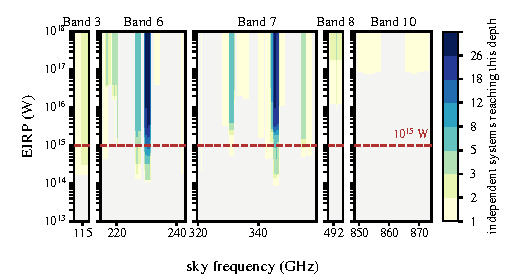
\includegraphics[width=\columnwidth]{figures/completeness_map.pdf}
\caption{Where the experiment could have found something. Shading gives the
number of independent systems in which an unresolved carrier of the plotted
EIRP at the plotted sky frequency would have been recovered nine times in
ten \emph{in a single epoch}; unshaded means none. That is a recovery
completeness and not a probability of confirmation: confirmation requires a
second independent epoch covering the same cell, which
Figure~\ref{fig:confcov} maps and which no amount of transmitted power can
supply. One panel per populated ALMA band, with panel widths in proportion
to the frequency each contributes: the \CvUnionA\,GHz Class~A union is
\CovNIslands{} disjoint islands across \DomAFreqLo--\DomAFreqHi\,GHz, which
a continuous abscissa would draw as hairlines. The dashed line is
$\CovEirpRefTex$\,W.}
\label{fig:covmap}
\end{figure}

The conventional measure for comparing programmes is the continuous-waveform
transmitter figure of merit of \citet{Enriquez2017},
$\mathrm{CWTFM}=\zeta_{\rm AO}\,\mathrm{EIRP}_{\rm min}/
(N_{\star}\nu_{\rm rel})$ with $\nu_{\rm rel}=\Delta\nu/\nu_{\rm mid}$,
smaller being better. Those programmes quote $\mathrm{EIRP}_{\rm min}$ at a
bare detection threshold, and not at the same one: \citet{Enriquez2017} quote
at $\mathrm{S/N}=\FomLitSnrEnriquez$ and \citet{Margot2023} at
\FomLitSnrMargot, where this search triggers at five
(Table~\ref{tab:litthresh}). The measure is linear in
$\mathrm{EIRP}_{\rm min}$, so putting every programme on the common footing
of five moves the published values --- \FomLitEnriquez{} becomes
\FomLitEnriquezFive{} and \FgLitMargot{} becomes \FgLitMargotFive{} --- and
it runs against this survey, making the comparison programmes deeper than
their own papers report. \citet{Margot2023} publish no CWTFM; that value is
the same expression on the three quantities they do give, \FomMargotN{}
stars, \FomMargotLo--\FomMargotHi\,GHz and
$\mathrm{EIRP}>\FgMargotEirp$\,W. This experiment takes no such factor, and
on that common footing, with $N_{\star}=\NSysClassA$ and
$\nu_{\rm rel}=\FomNuRel$, the Class~A experiment is $\SzCwtfmBareWorst$ on
the sample's largest threshold power and $\SzCwtfmBareMed$ on the median
system, a gap of $\FgGapBarePub$ from the published Enriquez value that
widens to $\FgGapBareFive$ once that value is rescaled with the rest.
On the $\mathrm{EIRP}_{90}$ adopted everywhere else here the same two
figures of merit are $\FomCwtfmWorst$ and
$\FomCwtfmMed$. Nearly all of
the difference is the product $N_{\star}\nu_{\rm rel}$: this is a far smaller
haystack than a wideband centimetre survey of thousands of stars, and the
measure compares surveys rather than estimating occurrence rates.

\subsection{What this experiment excludes, and what it does not}
\label{sec:excludes}

\noindent\emph{The signal these limits describe.} Every limit here applies to
one kind of signal: an unresolved carrier at the stellar position, confined to
a single \ChanLoA--\ChanHiA\,kHz channel, lying outside the molecular-line
mask, radiating while one of the archival blocks is on sky, and changing
frequency linearly at no more than its own window's ceiling,
\DriftCeilLo--\DriftCeilHi\,nHz. Such a carrier would
have produced a crossing nine times in ten above the $\mathrm{EIRP}_{90}$ of
\S\ref{sec:pninetysel}, and none survived toward any of the \NSysClassA{}
systems the carrier search covers. Four conditions
bound it as sharply as power does: the coverage is sparse and
inherited (Fig.~\ref{fig:covmap}), the median system covered over only
\SysUnionAMed\,GHz; the drift grid reaches an acceleration that contains every
known planet of the sample but one, but not a transmitter on a rapidly
rotating body (Fig.~\ref{fig:accel}); emission broader than one channel is
removed with the spectral baseline; and a carrier on for part of a block comes
back at that fraction of its amplitude, while one absent throughout is not
constrained at all.

\noindent\emph{Recurrence applies over a far smaller domain.} A
crossing is not a detection (Table~\ref{tab:quantities}), and where the archive
observed only once no power makes one. Recurrence could be tested for
\RcConfSysDay{} of the \NSysClassA{} systems at a frequency the first epoch
covered (\S\ref{sec:confirmability}); for the other \RcNoRepSys{} the
confirmation completeness is zero. Where it does apply, the test has power
only against a carrier as strong as the trigger demands of the repeat, so a
shallow repeat excludes nothing (\S\ref{sec:etacrv}).

\noindent\emph{The result is a non-detection and not an exclusion of
persistent transmitters.} An exclusion is read at the one cell the first
epoch predicts, so the transmitter it tests is one that comes back to that
cell, and four restrictions on that model are
ours. A transmitter operating intermittently need not have been radiating
during the second block. A second block need not cover the frequency at all,
and over about half the searched bandwidth none does
(\S\ref{sec:mmdifferent}). Orbital motion moves the carrier in the star's own
frame, and the interval the test permits is only half a channel, which an
orbit at 1\,au can carry a transmitter out of between the epochs
(\S\ref{sec:etacrv}). A transmitter may also change frequency deliberately,
and nothing here addresses that. Outside the adopted criterion, then, nothing
is excluded: neither emission inside the
$\pm\MaskHalfKms$\,km\,s$^{-1}$ molecular-line mask at any strength, nor any
emission from the \NGaiaCensus{} stars within 40\,pc that ALMA has not
observed, which is almost all of them.

\noindent\emph{An illustrative engineering benchmark.} A \BenchDiam\,m dish
radiating \BenchPowerMW\,MW at \BenchFreqGHz\,GHz with an aperture efficiency
of \BenchEta{} has a directive gain $G=\eta(\pi D\nu/c)^{2}=\BenchGain$ and so
an EIRP of $\BenchEirp$\,W, a depth this survey reaches for \BenchNSysA{} of
the \NSysClassA{} Class~A systems. The same gain makes its beam
$\Omega=4\pi/G=\BmOmegaSr$\,sr, \BmArcsec{} arcsec across and illuminating
$\BmSkyFrac$ of the sky. EIRP is not transmitter power --- the same megawatt
radiated isotropically would be $10^{6}$\,W --- so these limits apply to
beamed transmitters whose beam contains the Solar System.

\noindent\emph{Two blind spots.} The search forms Stokes~$I$ as
$(\mathrm{XX}+\mathrm{YY})/2$, which retains the full intensity of a circularly polarised
carrier; what is lost is not sensitivity but the discrimination polarisation
would offer against unpolarised astrophysical emission, because ALMA's feeds
are linear and the circularity lies in the cross-hands, which this analysis
does not extract. And the frequency coverage is the archive's and not a choice; none
of the ``magic frequency'' arguments that have guided centimetre-band searches
falls in an ALMA band.

\subsection{What a dedicated ALMA technosignature experiment should do
differently}
\label{sec:future}

A purpose-built experiment on the same telescope would be far stronger, and
the changes it needs follow from the limitations above. \emph{Channelise
finely everywhere:} the \NCoarse{} coarse-channel windows cannot carry a
carrier search at all.
\emph{Choose the targets and the frequencies:} an archive weighted toward
dusty discs is the worst case for molecular-line confusion, the M~dwarfs that
dominate the nearby habitable-zone planet census are the least covered, and
windows placed deliberately away from the bright transitions would recover
most of the \MkMaskAGHz\,GHz of the \CvUnionA\,GHz Class~A union that the
mask costs, \MkMaskAPct{} per cent of it --- all three are decisions a
proposal can simply reverse. \emph{Repeat the epochs on purpose, at the same
tuning:} two or three visits separated by days and by years turn a crossing
into a testable claim, and the separation is a scheduling constraint rather
than extra sensitivity; Fig.~\ref{fig:confcov} is what its absence costs.
\emph{Retain the visibilities:} rotating the phase centre to the star leaves a
genuine point source entirely in the real part of the visibility. That asks
whether the data contain a source \emph{where the star is}, which is a
stronger question than any rank
against neighbouring positions in an image.

%% ---------------------------------------------------------------------
%% REQUEST (06_discussion owner -> integrator). Consequences of this pass.
%% None of them is in a file I own; each is also written up as a numbered
%% entry in referee_r10/INTEGRATION_QUEUE.md.
%%
%% Q1. LABELS. sec:newspace, sec:excludes and sec:discussion are unchanged.
%%     sec:exposure and sec:parallax are GONE (see Q2, Q3); no file refers
%%     to either. sec:lessons is renamed sec:mmdifferent; the benchmark is
%%     a labelled paragraph inside sec:excludes, which is where \S2 now points.
%% Q2. THE OMITTED ANNUAL PARALLAX subsection is deleted from the Discussion
%%     under the ruling that the correction is applied rather than stated.
%%     The statement must now be made exactly once, where it is applied, in
%%     Section 5.1 / Appendix A. Macros \PxNWin, \PxLossMedPct,
%%     \PxLossMaxPct, \PxNGtTen and \PxNSysCorr are no longer referenced by
%%     any file I own and retire_macros.py will drop them unless that
%%     statement cites them.
%% Q3. THE ON-SOURCE TIME subsection (two offsetting bookkeeping biases) is
%%     deleted here as reproducibility detail. It belongs in Appendix A.
%%     Macros \TruncNBlocks, \ExpNBlocks, \TruncNWin, \TruncNStars,
%%     \TruncHoursLost, \TruncPctSurvey, \TruncGainMed, \OcOldMax,
%%     \OcNewMax, \ExpNetLo, \ExpNetHi are orphaned by that deletion.
%% Q4. THE MASON MATCHED-RECEIVED-FLUX COMPARISON is now made once, in
%%     Section 2, as that section's own request asked. \FluxSelMatchMed and
%%     \FluxSelMedRatio are unused.
%% Q5. THE BENCHMARK must stop being quoted as a headline result elsewhere:
%%     it is now an explicitly illustrative example in Section 6.3.
%%     Remove it from the abstract, from Section 5 and from conclusion 3,
%%     each of which should quote the EIRP_90 limit alone.
%% Q6. CONCLUSION 1 states that \UnionBandThree GHz of the searched range
%%     lies inside the interval covered by centimetre-wave programmes. It
%%     does not; that is the Band 3 union inside the Wright et al. haystack
%%     AXIS. Replacement text is in the integration queue.
%% Q7. Figure fig:covmap is new and is paid for: the millimetre-motivation
%%     paragraph (duplicated from Section 1), the Mason flux comparison, the
%%     parallax subsection and the exposure subsection are all deleted here.
%% ---------------------------------------------------------------------
